\documentclass[pre,twocolumn,groupedaddress,showpacs,showkeys,amsmath,amssymb,floatfix]{revtex4-1}

\usepackage{graphicx}
\usepackage{dcolumn}
\usepackage{bm}

\usepackage{subfigure}

\newcommand{\avg}[1]{\ensuremath{\left< #1 \right>}}
\newcommand{\avgR}[1]{\ensuremath{\left[ #1 \right] _{\mathrm{avg}}}}
\newcommand{\abs}[1]{\ensuremath{\left\vert#1\right\vert}}
\newcommand{\brac}[1]{\ensuremath{\left(#1\right)}}

% \newcommand{\change}[1]{{\bf #1}}
% \newcommand{\changeAH}[1]{{\bf #1}}

\begin{document}

    \title{Critical Temperature of the Ising Ferromagnet on Proximity Graphs derived from Square Lattices by Site Displacement}
    \author{Hendrik Schawe}
    \email{hendrik.schawe@uni-oldenburg.de}
    \author{Christoph Norrenbrock}
    \email{christoph.norrenbrock@uni-oldenburg.de}
    \author{Alexander K. Hartmann}
    \email{a.hartmann@uni-oldenburg.de}
    \affiliation{Institut f\"ur Physik, Universit\"at Oldenburg, 26111 Oldenbug, Germany}
    \date{\today}

    \begin{abstract}
        We perform Monte Carlo simulations to determine the critical temperatures
        of Ising Ferromagnets (IFM) on proximity graphs with different underlying
        node sets, which can be governed by a parameter $\sigma$.
        The coupling strengths arise from the Euclidean distance
        between coupled spins.
        The simulations are carried out on graphs with \(N=16^{2}\) to \(N=128^{2}\)
        nodes utilizing the Wolff cluster algorithm and parallel tempering in a
        wide temperature range around the critical point to measure
        the Binder cumulant as means to obtain the critical temperature.
        The critical temperatures are shown to depend mainly on the average degree
        and the type of the underlying proximity graph.
        We further verify using finite-size scaling methods that the IFM on proximity
        graphs is in the same universality class as the IFM on a two-dimensional
        square lattice.
    \end{abstract}

    % TODO: recherchieren und ändern
    %~ \pacs{64.60.ah}
    \maketitle

    \section{Introduction}
        The Ising model of ferromagnetism \cite{Ising1925} is one of the
        most extensively studied models in statistical mechanics, because it
        features a continuous phase transition while being simple.
        The model consists of discrete variables, called spins, which can be in
        one of two different states.
        The neighbor relationships, which define the interactions of spins, can be expressed by graphs and
        thus there is a constant interest in the critical behavior of this model
        on different graph ensembles. The research provides the whole range
        from analytical results for regular lattices \cite{Onsager1944,Wannier1945}
        to numerical results for complex networks \cite{Aleksiejuk2002260,Herrero2002SmallWorld,Herrero2004ScaleFree,Herrero2015ScaleFree}.

        An important graph is the Delaunay triangulation that finds application
        in, e.g., finite volume methods.
        For a system of randomly placed spins on a two-dimensional surface
        with neighbor relationships derived from a Delaunay triangulation,
        the critical temperature has been obtained
        and it has been confirmed that it is in the same universality class as the
        two-dimensional Ising model on a square lattice \cite{Janke1994,Lima2000,Lima2008}.
        This article extends the former research to other
        irregular lattices, namely the Relative Neighborhood graph (RNG) and
        Gabriel graph (GG), which are subgraphs of the Delaunay triangulation
        and belong to the family of \emph{proximity graphs}.
        The objective of proximity graphs is to connect nodes which are
        spatially close to each other, hence they are suited
        to generalize problems defined on regular lattices with nearest neighbor
        relationships.
        This family of graphs finds application in geographic variation studies in
        biology \cite{Sokal1978,Sokal1980,Selander1975}, as potential candidates for ``virtual backbones'' in ad-hoc
        networks \cite{Kuhn2003,Bose2001,Santi2005,Karp2000,jennings2002topology}
        and in machine learning and pattern recognition \cite{bhattacharya1981application}.
        Also, their statistical properties have been under scrutiny recently \cite{RNGCell,norrenbrock2014percolation}.

        Here, we consider an ensemble depending on a tunable parameter $\sigma$.
        By changing this parameter we can interpolate the configurations
        between nodes on a square lattice and nodes distributed by a Poisson point process.
        For any node set the construction rule of a proximity
        graph defines the corresponding edge set.
        We measure the critical temperatures for a range of $\sigma$ and find
        a power-law relationship for the GG between the critcal temperature and
        the average degree, for the RNG we cannot observe a power law.
        Additionally we verify that the universality class does not change by
        varying $\sigma$.

        In Sec.~\ref{sec:model} proximity graphs and the Ising model
        are explained. Sec.~\ref{sec:results} shows the
        details and results of our simulations. Sec.~\ref{sec:conclusion}
        closes this article with the conclusion and an outlook.


    \section{Model}
        \label{sec:model}
        \subsection{Proximity Graphs}
        \label{ssec:graphtypes}
            A graph \(G(V,E)\) consists of a set of nodes \(V\) and edges \(E \subset V^{2}\).
            Two nodes connected by an edge are called neighbors.
            Proximity graphs are defined in a metric space. In this article a
            two-dimensional space with the Euclidean metric is chosen, because
            it is the most common case and easy to visualize, though in principle
            every metric in any dimension can be used.

            The \emph{Relative Neighborhood graph} (RNG) \cite{Toussaint1980} is
            a proximity graph. Two nodes \(i\) and \(j\) with distance $d_{ij}$
            will be connected, if no other node is in their \emph {lune}. The lune
            is defined as the intersection of two circles with radius \(r =
            d_{ij}\) and centers on \(i\) and \(j\). That means that the edge
            $\{i,j\}$ is part of the graph, if the condition
            \begin{align*}
                d_{ij} &\le \max\left\{ d_{ik}, d_{kj} \right\} &\forall k \in V\setminus\{i,j\}
            \end{align*}
            is fulfilled. See also the hatched region
            in Fig.~\ref{fig:lunes}. An example is given in Fig.~\ref{sfig:lunes:rng}.

            \begin{figure}[htbp]
                \centering
                \subfigure[]{
                    \label{sfig:lunes:def}
                    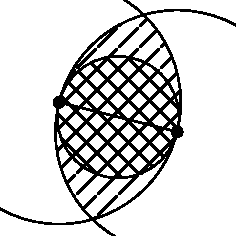
\includegraphics[width=0.14\textwidth]{images/GG_RNG_def}
                }
                \subfigure[]{
                    \label{sfig:lunes:rng}
                    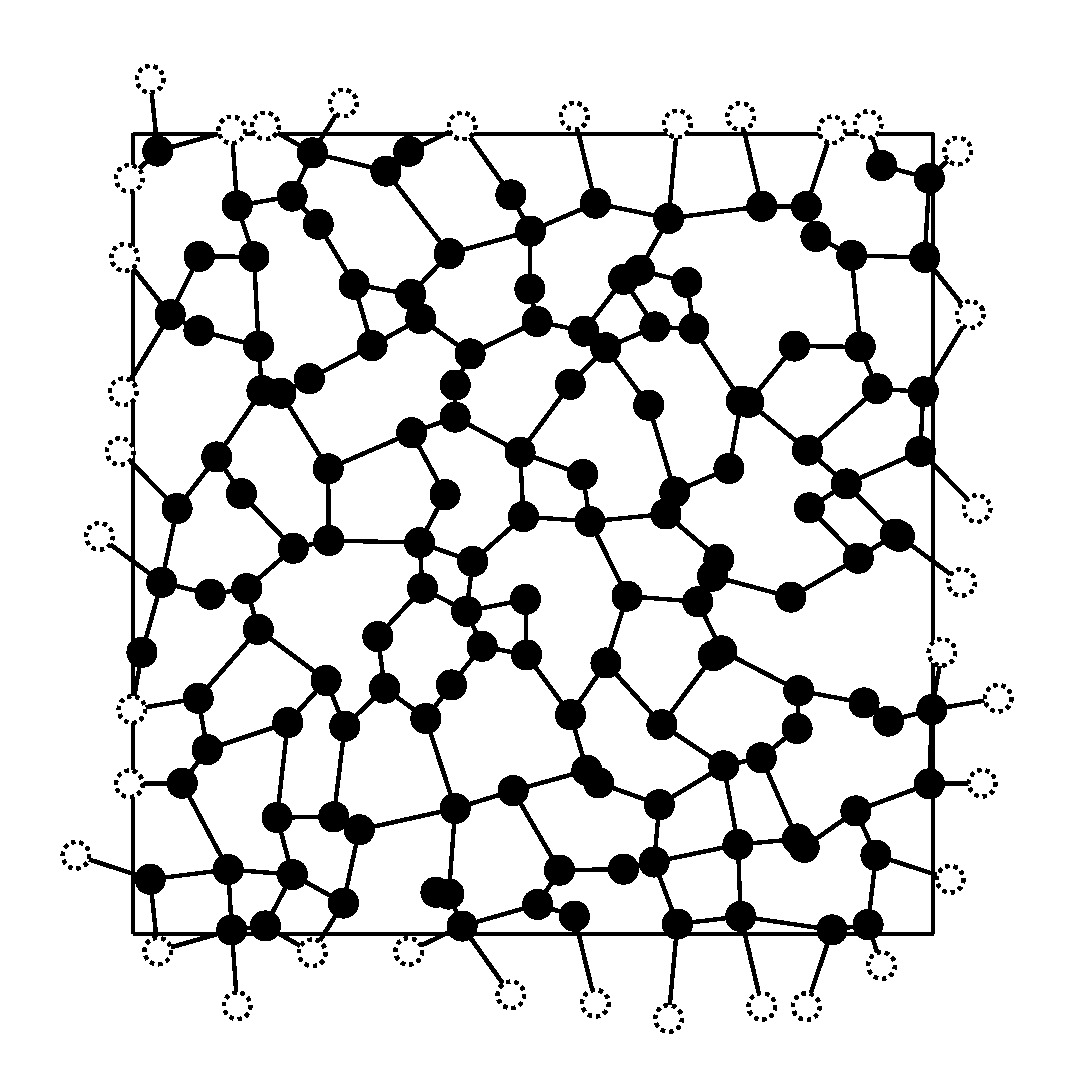
\includegraphics[width=0.14\textwidth]{images/RNG/L12S03}
                }
                \subfigure[]{
                    \label{sfig:lunes:gg}
                    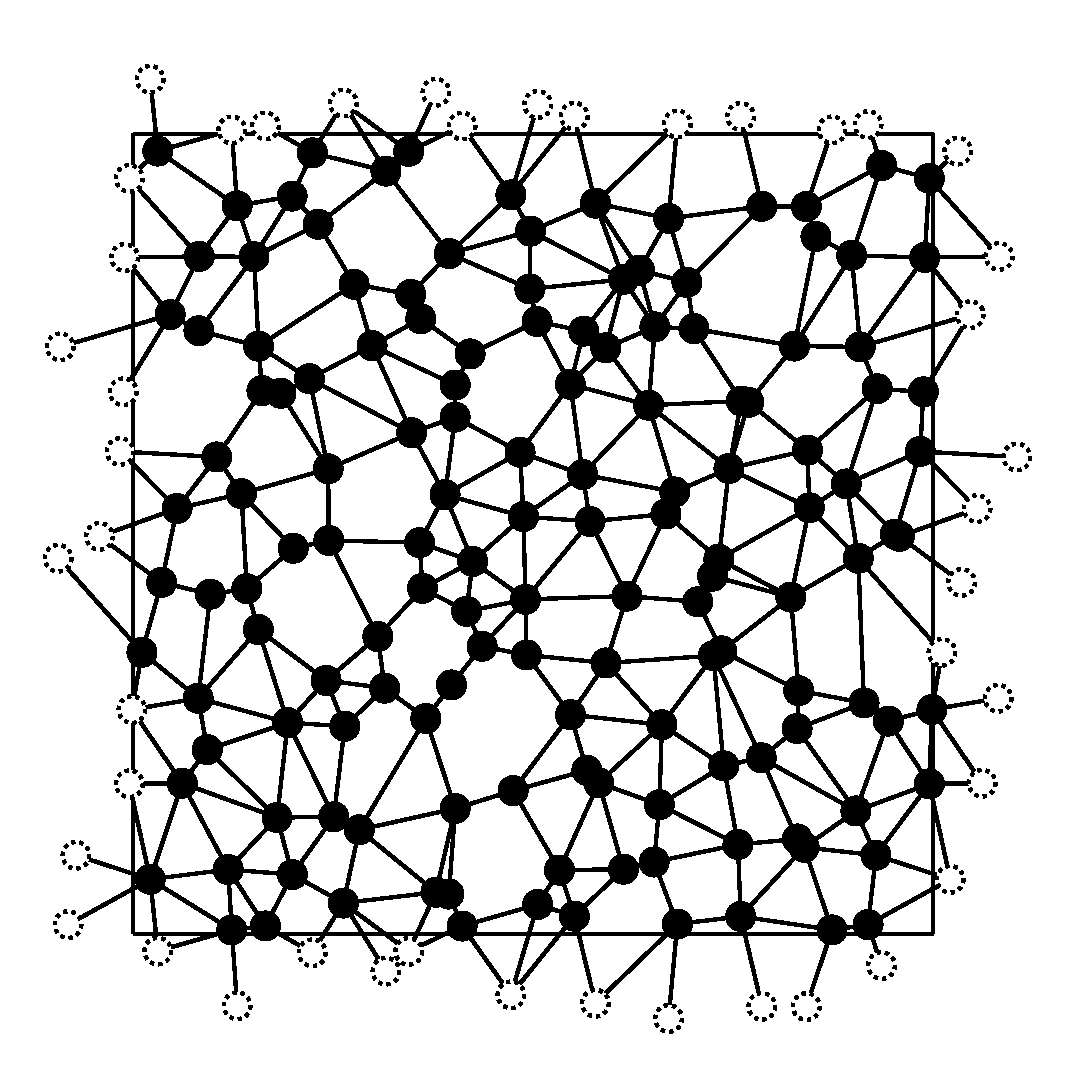
\includegraphics[width=0.14\textwidth]{images/GG/L12S03}
                }
                \caption[Gabriel and Relative Neighborhood Graph]
                {
                    \subref{sfig:lunes:def} Lunes, which define whether an edge
                        exists, of RNG (hatched region) and GG (cross hatched region).
                        It is evident from this sketch that the GG is a supergraph
                        of the RNG. If there is an edge in the RNG, the hatched
                        region contains no node, then of course also the double
                        hatched region contains no node and thus this edge appears
                        also in the GG. So every egde of the RNG is also present
                        in a GG on the same set of nodes.
                    \subref{sfig:lunes:rng} Example of a RNG on periodic
                        boundary conditions.
                    \subref{sfig:lunes:gg} Example of a GG on
                        periodic boundary conditions. Periodic nodes are dashed.
                }
                \label{fig:lunes}
            \end{figure}

            The \emph{Gabriel graph} (GG) \cite{Gabriel1969} is a subgraph
            of the Delaunay triangulation \cite{Delaunay1934,Katajainen}
            (DT), i.e., for the same set of nodes \(V\) the edge set of the
            DT is a superset of the edge set of the GG. Two nodes \(i\) and
            \(j\) with distance \(d_{ij}\) will be connected with an edge,
            if a circle with its center on half way between \(i\) and \(j\)
            and radius \(r = \frac{d_{ij}}{2}\) contains no other nodes, i.e., the
            condition
            \begin{align*}
                d^{2}_{ij} &< d^{2}_{ik} + d^{2}_{kj} &\forall k \in V\setminus\{i,j\}
            \end{align*}
            is fulfilled. See
            also the cross hatched region from Fig.~\ref{sfig:lunes:def}. An
            example is given in Fig.~\ref {sfig:lunes:gg}. Note that the
            lune of the GG is completely enclosed in the lune of the RNG,
            therefore the RNG is a subgraph of the GG.

            To construct these graphs there is an algorithm with
            a time complexity of \(\mathcal{O}(N \log N)\) for nodes on a two
            dimensional plane \cite{RNGCell}.

        \subsection{The Ising Model}
        \label{ssec:model}
            Commonly, the IFM is studied on a square lattice with lateral length
            \(L\) and \(N=L^2\) nodes with periodic boundary conditions.
            Each node $i$ has an Ising spin \(s_i \in \{-1,+1\}\) and interacts with its
            nearest neighbors described by the Hamiltonian
            \begin{equation}
                \mathcal{H} = - \sum_{\avg{i,j}}J_{ij}s_{i}s_{j}.
                \label{eq:hamiltonian}
            \end{equation}
            \(\avg{i,j}\) refers to nodes \(i\) and \(j\) which are
            nearest neighbors, i.e., they are connected by an edge.
            The coupling strength between \(i\) and \(j\) is given by
            \(J_{ij}\).

            In this article the nodes of the square lattice are
            displaced, introducing geometric disorder resulting in a non-regular graph
            structure.
            The displacement is randomly Gaussian distributed with standard
            deviation \(\sigma\), i.e., the \(x\) and \(y\) coordinates of the
            nodes are displaced by random \(\Delta x\) and \(\Delta y\) drawn
            from a Gaussian distribution with zero mean.
            In the following, \(\sigma\) will be called \emph{disorder parameter}.
            If we took ``nearest neighbor" in the Euclidean meaning, most nodes
            would only have one nearest neighbor after the
            displacement. If only the edges between these neighbors remained,
            the lattice would collapse to many very small clusters. If, on the
            other hand, all edges remained as they were before the displacement,
            edges might cross each other -- at least for big displacements.
            The crossing of edges would destroy the planar character of the graph.
            To avoid this, a new edge set will be established after the displacement
            to form a proximity graph. The influence of $\sigma$ on the
            structure of a proximity graph is shown in Fig.~\ref{fig:RNG_sigma}
            for a RNG.
            \begin{figure}[htb]
                \centering
                \subfigure[$\sigma = 0.09$]
                {
                    \label{sfig:RNG_sigma:0.09}
                    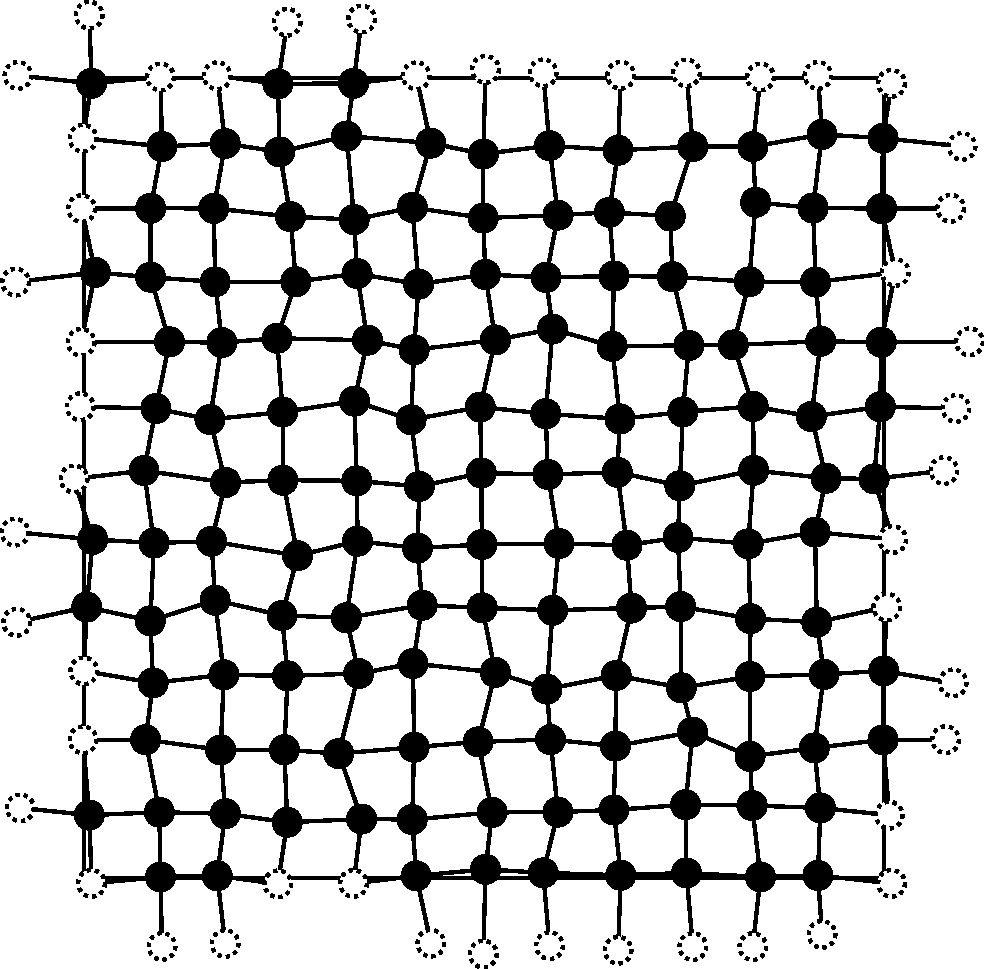
\includegraphics[width=0.14\textwidth]{images/RNG/out009}
                }
                \subfigure[$\sigma = 0.15$]
                {
                    \label{sfig:RNG_sigma:0.15}
                    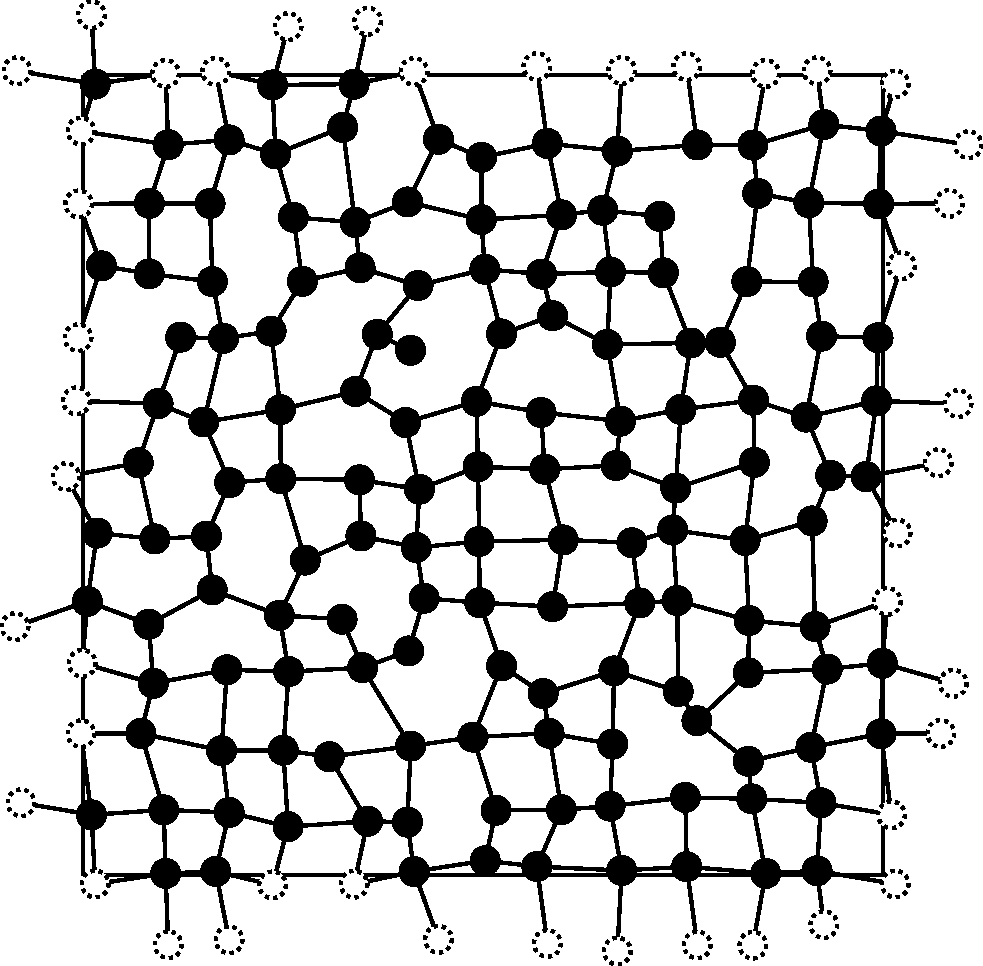
\includegraphics[width=0.14\textwidth]{images/RNG/out015}
                }
                \subfigure[$\sigma = 0.21$]
                {
                    \label{sfig:RNG_sigma:0.21}
                    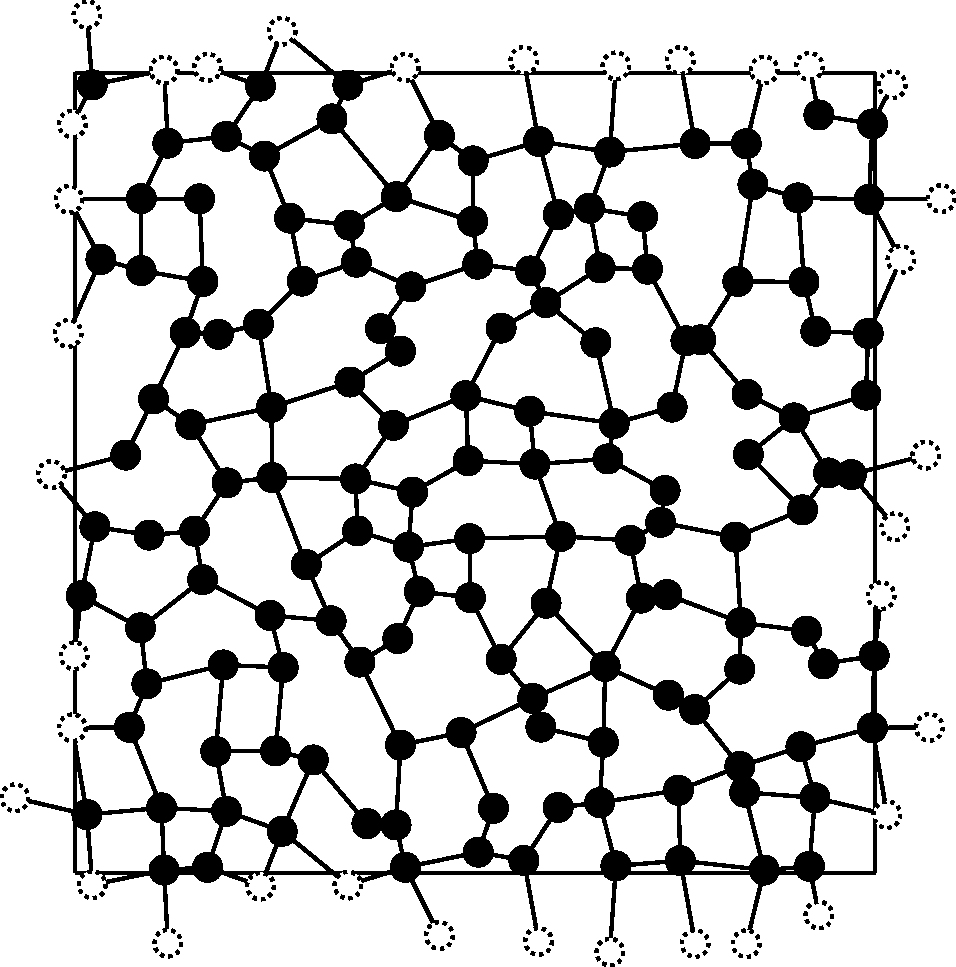
\includegraphics[width=0.14\textwidth]{images/RNG/out021}
                }
                \caption[Examples of RNG for different $\sigma$]
                {
                    Examples of proximity graphs (more precise, Relative Neighborhood
                    graph see Sec. \ref{ssec:graphtypes}) for different values of $\sigma$.
                    Connections which cross a periodic boundary are indicated
                    by edges which connect a solid node to a dashed node.
                }
                \label{fig:RNG_sigma}
            \end{figure}
            The coupling constants \(J_{ij}\), i.e., edge weights, depend on the
            geometric distance between the connected pair of nodes. More precise,
            the weight of an edge is
            \begin{equation}
                E_{ij} = J_{ij} = \mathrm{e}^{\alpha (1-d_{ij})},
                \label{eq:coupling}
            \end{equation}
            where \(d_{ij}\) is the Euclidean
            distance between node \(i\) and \(j\). Following Ref.~\cite{Lima2000}
            the free parameter \(\alpha\) is set to \(\alpha = 0.5\).
            Note that for \(\sigma = 0\) the resulting \(d_{ij} = 1\) and therefore
            \(J_{ij} = 1\) for every edge $\{i,j\}$. Consequently, in this case
            the graph is a common square lattice.


    \section{Results}
        \label{sec:results}
        The results are obtained through Monte Carlo simulations. For each
        sweep \(N\) single spin flip Metropolis updates \cite{Metropolis1953},
        one Wolff cluster update \cite{Wolff1989} and one
        parallel tempering swap \cite{ParallelTempering1986} are performed.
        For every system size $L \in \{16,32,64,128\}$ and 19 different values of
        $\sigma \in [0,1.2]$ on $100$ different realizations at least $5000$
        independent measurements are taken in equilibrium.\\
        Since it is not known beforehand, where the critical temperatures \(T_c\)
        are located, the Wolff cluster algorithm is used at every
        temperature. Albeit the efficiency of the algorithmic procedure was
        not examined for every temperature, the speed up near criticality
        should be worth the moderate slow down at other temperatures.\\

        It is not expected that the universality class depends on the graph
        structure unless the dimension is changed.
        To proof this, the critical exponents are determined by a finite-size
        scaling (FSS) analysis using the well kown scaling bahaviors of the
        magnetization, the susceptiblity and the Binder cumulant
        in an automated and reproducable way using the
        method from Ref.~\cite{autoscale2009}.
        In Fig.~\ref{fig:collapse}
        \begin{figure}[htb]
            \includegraphics[scale=1]{plots/col_s1_sus}
            \caption[Examples of Determining Critical Temperature and Exponents]
            {
                Example for a collapse of the susceptiblity \(\chi\) on a RNG at
                \(\sigma = 1\) to get the corresponding critical exponent $\gamma$.
                The same procedure is used on the Binder cumulant $g$ and the
                magnetization $|m|$ to determine the critical exponents
                \(\nu\) and \(\beta\) and the critical temperature \(T_c\).
                The inset shows the same data with unscaled axes.
            }
            \label{fig:collapse}
        \end{figure}
        a data collapse at $\sigma = 1$ for the susceptiblity
        \[\chi = \frac{N}{T}\brac{\avgR{\avg{m^2}}-\avgR{\avg{m}}^2}\]
        with $\avg{\cdot}$ being the thermal average and $\avgR{\cdot}$ being the
        average over the random realizations, is plotted.
        All obtained values for different $\sigma$ are visualized in Tab.~\ref{tab:critExp}
        \begin{table}[htb]
            \begin{ruledtabular}
                \begin{tabular}{l l l l l l}
                     & \multicolumn{1}{c}{\(\sigma\)} & \multicolumn{1}{c}{\(T_c\)} & \multicolumn{1}{c}{\(\nu\)} & \multicolumn{1}{c}{\(\gamma\)} & \multicolumn{1}{c}{\(\beta\)}\\
                    %~ \colrule
                    \hline
                    exact        & 0   & 2.2691... & \(1\)    & \(1.75\) & \(0.125\)\\
                    %~ \colrule
                    \hline
                    RNG          & 0.0 & 2.2688(7) & 1.00(1) & 1.74(1) & 0.125(1) \\
                                 & 0.1 & 2.2053(6) & 0.99(1) & 1.75(1) & 0.128(3) \\
                                 & 0.2 & 1.6265(19)& 1.02(2) & 1.76(1) & 0.122(7)\\
                                 & 0.5 & 1.2825(9) & 1.01(2) & 1.75(2) & 0.128(8)\\
                                 & 1.0 & 1.2125(5) & 1.01(1) & 1.76(1) & 0.125(6)\\
                    %~ \colrule
                    \hline
                    GG           & 0.0 & 2.2688(6) & 1.00(1) & 1.74(2) & 0.127(4)\\
                                 & 0.1 & 2.8944(43)& 1.00(1) & 1.75(1) & 0.135(6) \\
                                 & 0.3 & 2.5281(27)& 1.03(3) & 1.72(2) & 0.118(11)\\
                                 & 0.5 & 2.2388(9) & 1.01(1) & 1.75(1) & 0.125(11)\\
                                 & 1.0 & 2.1275(20)& 1.04(3) & 1.75(2) & 0.125(15)\\
                \end{tabular}
            \end{ruledtabular}
            \caption[Critical Exponents for Different $\sigma$]{
                Critical exponents for different values of \(\sigma\). A finite size
                scaling analysis was performed to determine the critical
                exponents \(\beta, \gamma, \nu\) and the critical temperature
                \(T_c\). The errors for \(\beta\) and \(\gamma\) are estimated
                with the method from Ref.~\cite{autoscale2009}. The errors of
                \(\nu\) and \(T_c\) are the standard deviation of three obtained
                values through different collapses. The critical exponents
                are in reasonable agreement with the exact known values for the 2D Ising
                universality class. The critical temperatures $T_c$ are shifting
                as expected.
            }
            \label{tab:critExp}
        \end{table}
        and are within errorbars consistent with the exactly known values for the
        square lattice IFM.
        A newer method \cite{chiCollapse,Hartmann2013} to test whether two models are in
        the same universality class is the analysis of the two-point finite-size
        correlation function
        \[\xi = \frac{1}{2\sin\brac{\abs{\vec{k}_{\mathrm{min}}}/2}} \sqrt{\frac{\chi(\vec{0})}{\chi(\vec{k}_{\mathrm{min}})} - 1}\]
        where $\vec{k}_{\mathrm{min}}=(2\pi / L, 0)$ and $\chi(\vec{k})$ is the wave vector
        dependent susceptiblity
        \[\chi(\vec{k}) = \avgR{\avg{\abs{\brac{\frac{1}{N}\sum_j s_j \exp(ikx_j)}^2}}}\]
        which is in this case only evaluated over one direction thus $x_j$ is the
        position of the node in the x-direction.

        \begin{figure}[htbp]
            \centering
            \includegraphics[scale=1]{plots/Binder_over_Correlation_All}
            \caption[Binder cumulant over two-point finite-size correlation function divided by system size]
            {
                Binder cumulant $g$ over two-point finite-size correlation function
                divided by system size $L$. The datapoints for different system sizes
                are drawn with different symbols, while the datapoints for different
                graph ensembles are drawn with different colors. Anyway, all points
                fall on one curve within errorbars.
                %~ The inset zooms into the plot to show that
                %~ all datapoints fall within errorbars onto one curve.
            }
            \label{fig:binderOverCorr}
        \end{figure}
        If the Binder cumulant
        \[g = \frac{3}{2}\brac{1-\frac{\avgR{\avg{m^4}}}{3\avgR{\avg{m^2}^2}}}\]
        is plotted over $\xi$ for different $\sigma$, $L$ and $T$ as shown in
        Fig.~\ref{fig:binderOverCorr}, all data points fall on the
        same curve, which confirms that this IFM on proximity graphs is in the
        same universality class as on the square lattice, i.e., $\sigma=0$.

        This study examines the critical temperatures $T_c$ for different values of $\sigma$.
        Therefore the knowledge that the Binder cumulants $g$ for different
        system sizes $L$ intersect at $T_c$ \cite{Binder1981} as shown in Fig.~\ref{sfig:Tc:binder}
        is used.
        \begin{figure*}[hbtp]
            \subfigure[]{
                \label{sfig:Tc:binder}
                \includegraphics[scale=1]{plots/binder}
            }
            \subfigure[]{
                \label{sfig:Tc:RNG}
                \label{sfig:Tc:GG}
                \includegraphics[scale=1]{plots/Tc_both}
            }
            \subfigure[]{
                \label{fig:TcK}
                \includegraphics[scale=1]{plots/K_sigma_inset_both}
            }
            \caption[Critical Temperature over Different Disorder Parameters]
            {
                \subref{sfig:Tc:binder} Critical temperatures \(T_c\) are obtained by finding the intersections
                of the Binder parameters $g$ for different system sizes $L$.
                \subref{sfig:Tc:RNG} They are plotted over different disorder parameters \(\sigma\).
                Interesting points are the jump and rise of the GG at small
                \(\sigma\) and the plateau on the RNG for small \(\sigma\).
                \subref{fig:TcK} The average degree \(K\) is plotted over $\sigma$ and
                the similarity to \subref{sfig:Tc:RNG} shows that the degree is the single
                most important influence on $T_c$. The inset shows that for the GG there
                is actually in good approximation a power-law relationship \(T_c = aK^b\)
                The upper curve is for an ensemble where the edges have unit weight and
                yields an exponent $b_1=1.321(1)$ with $\chi_{\mathrm{red}}^2 = 2.5$.
                The ensemble with length dependent weigth is the lower curve with
                $b = 1.305(2)$, $\chi_{\mathrm{red}}^2 = 4.9$.
                The bad $\chi_\mathrm{red}^2$ are caused by the region in the upper right,
                where $T_c$ is rising with $\sigma$ and hint at other influences.
            }
            \label{fig:Tc}
        \end{figure*}
        Since \(g\) is only measured for discrete values of \(T\),
        the points have to be interpolated to find the intersection. Therefore
        a \emph{cubic spline} \cite{press2007numerical} interpolation %footnote{created using the \texttt{scipy.interpolate} tools \cite{scipy2001}}
        is calculated for the measured points.
        %~ Cubic spline interpolation is a piece-wise fitting of polynoms of
        %~ degree three which are joined under the condition to be at least two
        %~ times continuously differentiable.
        %~ This interpolation type has the
        %~ advantage that it is only influenced by local points so that the
        %~ plateaus at low and high \(T\) do not influence the interpolation in
        %~ the vicinity of \(T_c\) -- in contrast to, e.g.\ an polynom fit of
        %~ degree 4, which has to be restricted to the vincinity of \(T_c\) to
        %~ yield meaningful results.
        An even better method would be the
        \emph{multiple histogram} method \cite[p. 219ff]{NewmanBarkema1999}.
        But the simple cubic spline interpolation seems to deliver results that
        are good enough, because the temperatures of the measurements are
        sufficiently near to each other. Also a cubic spline interpolation is
        far easier to obtain.

        \begin{figure}[hbtp]
            \includegraphics[width=0.15\textwidth]{images/GGEdgeAfter}
            \caption
            {
                Smallest movement of nodes in a square lead to a new edge across the
                facet. This effect leads to the discontinuity in Fig.~\ref{sfig:Tc:RNG} and
                Fig.~\ref{fig:TcK}.
            }
            \label{fig:GGEdgeAfter}
        \end{figure}
        The first oddity of the GG in Fig.~\ref{sfig:Tc:GG} which needs to be addressed is
        the jump of $T_c$ close to $\sigma = 0$, where it jumps from $T_c(0) = 2.269(1)$
        to $T_c(0.03) = 2.851(1)$ at the next measured temperature. This is easily explainable,
        because the square lattice at $\sigma = 0$ is a very special case for the
        GG and at smallest deviations from the square lattice new edges arise in
        the GG, this is visualized in Fig.~\ref{fig:GGEdgeAfter}. These new edges lead
        to a stronger coupling of spins such that the system stays ferromagnetic at
        higher temperatures.

        For large values of $\sigma$ the configurations approach the limit of a
        Poisson point process, hence $T_c$ approaches its limit value. Note that

        The critical temperature $T_c$ decreases with increasing $\sigma$, which
        is expected, since the number of edges decreases, which can be seen in
        Fig.~\ref{fig:RNG_sigma}. With loosely coupled spins, the temperature
        needed to disturb the ferromagnetic phase is lower than with strongly coupled
        spins.
        For the GG there is a power-law relationship between the degree $K$ and
        the critical temperature $T_c$ for both the distance dependent coupling constant
        and a constant $J=1$ as shown in the inset of Fig.~\ref{fig:TcK}. The exponents
        and goodness of fit are shown in the caption.
        Also here the square lattice $\sigma = 0$ is a special case, as it is incompatible with the
        power law. Also note that the points for small $\sigma$ in the top right of the
        inset are the ones wich worsen the goodness of fit. For the RNG this power law
        is not observable.
        A further interesting feature which highlights the immportance of the structure
        of the graph for the critical temperature is the fact that the square lattice
        has a different critical temperature than the GG in the Poisson point process
        limit although they share the same average degree of $K=4$. ($T_c/K$ als Wert einer Kante)
        %To quantify the influence of this, $T_c$ is plotted over the
        %degree $K$, i.e., the mean number of neighbors each spin has, in Fig.~\ref{fig:TcK}.
        %For a given graph type, $T_c$ can be derived approximately by a power law
        %from $K$. But there are deviations from this behavior, which reflect
        %at least the influence of the coupling constant $J$.


    \section{Conclusion}
        \label{sec:conclusion}
        This study shows that universality of the Ising model is preserved for
        irregular graphs on a wide range of configurations which are intermediate
        between the square lattice Ising model and a random Poisson point process.
        Also the critical temperature was measured over this range and determined
        that it shows approximately a power law behavior with the mean
        number of neighbors as the base and an exponent dependent on the
        graph type that defines the neighbor relationships.

        The next step would be the extension to three and higher
        dimensions, where the used proximity graphs are still well defined. It
        would also be worthwhile to study properties of the graph ensembles themselves,
        because -- to our knowledge -- they are mostly studied in 2D \cite{RNGCell}.


    \section{Acknowledgements}
        The simulations were performed at the HPC Cluster HERO, located at
        the University of Oldenburg (Germany) and funded by the DFG through
        its Major Research Instrumentation Programme (INST 184/108-1 FUGG)
        and the Ministry of Science and Culture (MWK) of the Lower Saxony
        State.
        The authors would also like to thank O. Melchert and T. Dewenter
        for the fruitful discussions.


    \bibliography{lit}
\end{document}
